%! TeX Program = lualatex
\documentclass{standalone}
\input{../tikz.tex.preamble}

\begin{document}
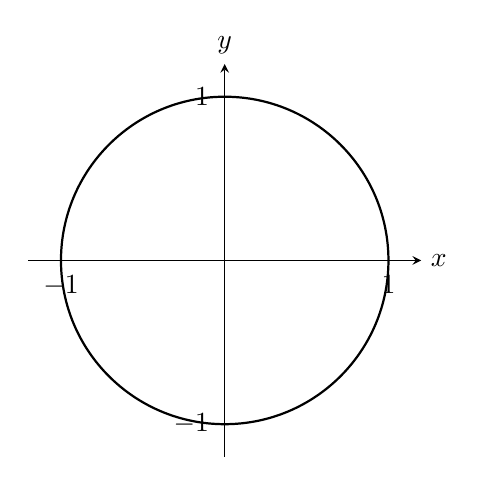
\begin{tikzpicture}[scale=1]
  \begin{axis}[
    axis lines = middle, % boxed, middle
    axis equal image,
    width = 3in,
    %
    % domain and range
    %
    xmin={-1}, xmax={1},
    ymin={-1}, ymax={1},
    enlargelimits=true,
    %
    % axis labels
    %
    xlabel={\(x\)}, xlabel style={anchor=west},
    ylabel={\(y\)}, ylabel style={anchor=south},
    label style={at={(ticklabel* cs:1)}},
    %
    % ticks
    %
    xtick={-1, 0, 1}, % xticklabels={},
    ytick={-1, 0, 1}, % yticklabels={},
    %
    % grid
    % none, major, minor, both
    grid=none, grid style={gray!20},
    % minor tick num=1, 
    % minor grid style={gray!20},
    % 
    % plot parameters
    %
    smooth, samples=100, no markers,
    ]
    % \draw[thick] (axis cs:0,0) circle (0.3);
    \draw[thick] (axis cs:0,0) circle (1);
    % \draw[thick] (axis cs:0,0) circle (2.2);
  \end{axis}
\end{tikzpicture}
\end{document}
